%\lesson{1}{wo 25 sep 2019 15:00}{Introduction}
%\begin{itemize}
%    \item Marco Zambon. TA: R. Storm
%    \item Literature: Tu, Lee
%    \item Exercises: Mondays. Look at exercises in advance. (part of exam is based on them)
%    \item Take home sheets: $2$, two weeks to solve them. 6/20. (solving together is allowed.) \emph{Write up by hand; no typing}
%    \item Exam: 16/20.
%        \begin{itemize}
%            \item 2 problems (closed book) (inspired by homework problems)
%            \item 2 questions (closed book)
%        \end{itemize}
%        Oral defence of this and one TH.
%    \item Time: 16:10 -- 18:00
%\end{itemize}
\linespread{1.35}
\chapter{Partial derivative and directional derivative}
\setcounter{section}{-1}
\section{Partial derivative}

we define partial derivative $\pdv{f}{x}$ and $\pdv{f}{y}$ as follows
\begin{definition}[partial derivative]
    $$\pdv{f}{x} \begin{pmatrix} a \\ b \end{pmatrix} = \lm{h}{0} \frac{f\m{a+h \\ b}- f \m{a \\ b}}{h} $$
    $$\pdv{f}{y} \begin{pmatrix} a \\ b \end{pmatrix} = \lm{k}{0} \frac{f\m{a\\ b+k}- f \m{a \\ b}}{k} $$

\end{definition}
\begin{eg}
    Let $f(x,y) = x^{3}y^{5} + e^{xy}\sin(2x+3y)$ then $$\pdv{f}{x} = 3x^{2}y^{5} + e^{xy}(2\cos(2x+3y)) + ye^{xy}(\sin(2x+3y))$$
\end{eg}

The partial derivative of $f$ measures the rate of change of $f$ in the direction of coordinate axis, i.e., in the direction of the standard basis vector $e_{1}, \dots e_{n}$
. Given any non-zero vector $v$, it is natural to consider the rate of change of $f$ in the direction of $v$.

\begin{definition}
    Let $U \subset \mc{R}^{n}$ be open and $a \in U$. We define the directional derivative of $f: U \mapsto \mc{R}^{m}$ at $a$ in the direction $v$ to be 
    $$D_{v}f(a) = \lm{t}{0}\frac{f(a+tv) - f(a)}{t}$$ 
    provided this limit exists.
\end{definition}
    
\begin{eg}
    Let $f: \mc{R}^{2} \mapsto \mc{R}$ by $$f(x,y) = \frac{|x|y}{\sqrt{x^{2}+y^{2}}}, \quad x \neq 0 \wedge f(0) = 0$$
    Then the directional derivative of $f$ at $0$ in the direction of unit vector $v = \m{v_{1}\\v_{2}}$
    $$D_{v}f(0) = \lm{t}{0}\frac{f(tv) - f(a)}{t}$$
    then it is trivial that this expression yields $|v_{1}|v_{2}$
\end{eg}
\begin{eg}
    Let $f = \m{x\\y\\z} = x^{2}y + e^{3x+y-z}$, and let $a = \m{1\\-1\\2}$ and $v = \m{2\\3\\-1}$. What is the directional derivative $D_{v}f(a)$?
    \\
    We define $\phi: \mc{R} \mapsto \mc{R}$ by $\phi(t) = f(a+tv)$. Note that $$\phi^{\prime}(0) = \lm{t}{0}\frac{\phi(t) - \phi(0)}{t} = \lm{t}{0}\frac{f(a+tv)-f(a)}{t} = D_{v}f(a)$$
    so we just calculate $\phi$ and compute its derivative at $0$
    $$\phi(t) = f\m{1+2t\\-1+3t\\2-t} = (1+2t)^{2}(-1+3t)+e^{10t}$$
    $$\phi^{\prime}(t) = 4(1+2t)(-1+3t)+3(1+2t)^{2} + 10e^{10t}$$
    from which we conclude $D_{v}(a) = \phi^{\prime}(0) = 9$
\end{eg}

\pagebreak
\section{Differentiability}
\begin{center}
    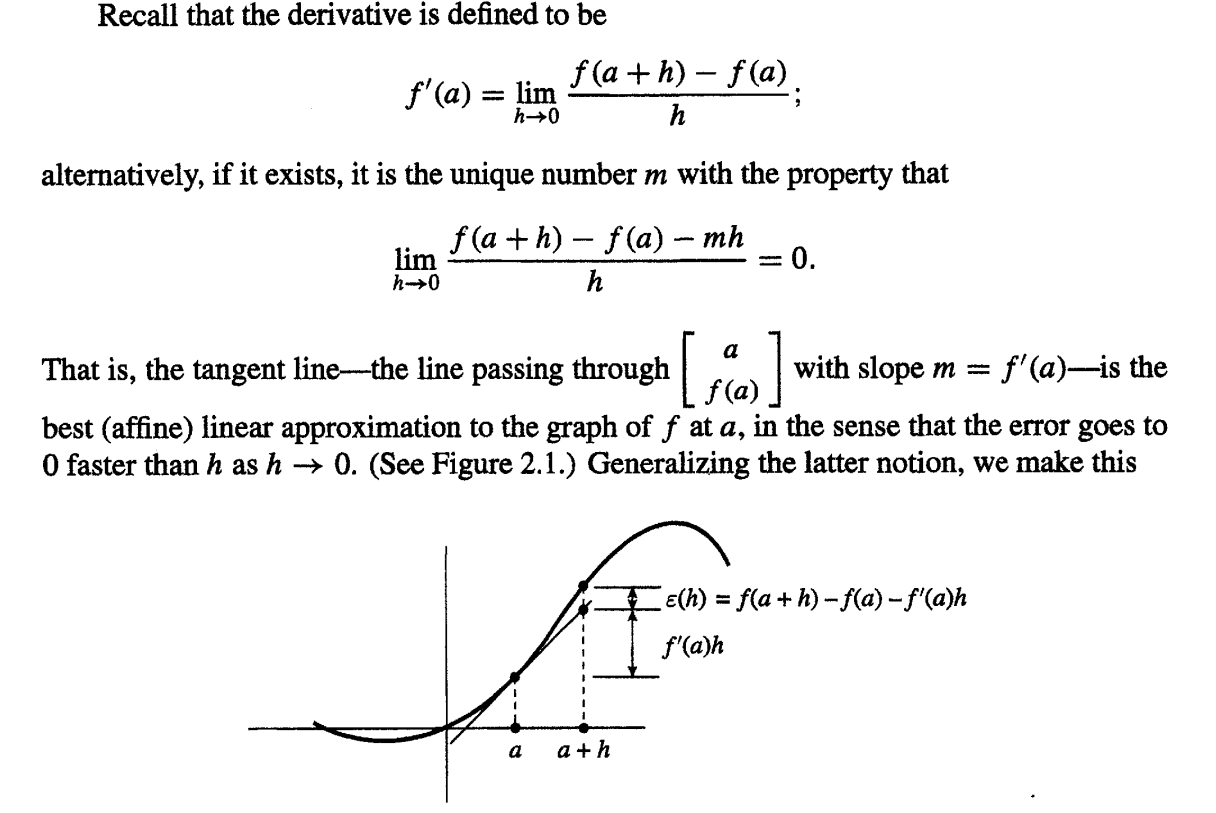
\includegraphics[totalheight=6cm]{Differential.png}
\end{center}
\begin{definition}
     Let $U \subset \mc{R}^{n}$ be open and $a \in U$. A function $f: U \mapsto \mc{R}^{m}$ is \textbf{differentiable} at $a$ if there is a linear map $Df(a): \mc{R}^{n} \mapsto R^{m}$ such that  $$\lm{h}{0}\frac{f(a+h)-f(a)-Df(a)h}{h} = 0$$ 
\end{definition}
This says that $Df(a)$ is the best linear approximation to the function $f - f(a)$ at $a$, in the sense that $f(a+h) - f(a) - Df(a)h$ converges faster than $h$.
\begin{remark}
    The derivative $Df(a)$, if exists, must be unique, the proof is skipped as it is trivial.
\end{remark}
\begin{prop}
    if $f: \mc{R}^{n} \mapsto \mc{R}^{m}$ is \textbf{differentiable} at $a$, then the partial derivatives $\pdv{f_{i}}{x_{j}}(a)$ exist and $$\m{Df(a)} = \m{\pdv{f_{i}}{x_{j}}(a)}$$
    The latter matrix is often called the Jacobian matrix of $f$ at $a$.
    
\end{prop}
\begin{proof}
    since we assume $f$ is differentiable at $a$, we know that there is a linear map $Df(a)$ with property that $$\lm{h}{0}\frac{f(a+h)-f(a)-Df(a)h}{||h||} = 0$$,
    for any $j = 1,...,n,$ we consider $h=te_{j}$ and let $t \mapsto 0$. Then we have $$0 = \lm{t}{0}\frac{f(a+te_{j}) - f(a) - Df(a)(te_{j})}{|t|} = 0$$
    Considering separately the cases $t>0$ and $t<0$, we find that $$\lm{t}{0^{+}}\frac{f(a+te_{j}) - f(a) - Df(a)(te_{j})}{|t|} = \lm{t}{0^{+}}\frac{f(a+te_{j}) - f(a)}{t} - Df(a)(e_{j})$$ 
$$\lm{t}{0^{-}}\frac{f(a+te_{j}) - f(a) - Df(a)(te_{j})}{|t|} = (-1)\lm{t}{0^{-}}\frac{f(a+te_{j}) - f(a)}{t} - Df(a)(e_{j})$$ 
so $Df(a)(e_{j}) = \lm{t}{0}\frac{f(a+te_{j}) - f(a)}{t} = \pdv{f}{x_{j}}(a)$
\end{proof}
\begin{prop}
    if $f: \mc{R}^{n} \mapsto \mc{R}^{m}$ is differentiable at $a$, then $f$ is continuous at $a$
\end{prop}
\begin{proof}
    Trivial, assume $f$ is differentiable at $a$ and deduce $\lm{x}{a}f(x) = f(a)$
\end{proof}
s
\section{Differentiation rules}
\begin{theorem}[Chain rule]
    Suppose $g: \mc{R}^{n} \mapsto \mc{R}^{m}$ and $f: \mc{R}^{m} \mapsto \mc{R}^{l}$, $g$ is differentiable at $a$ and $f$ is differentiable at $g(a)$. Then $f \circ g$ is differentiable at $a$ and 
    $$D(f\circ g)(a) = Df(g(a))Dg(a)$$
\end{theorem}
\begin{eg}
    Let $$f\m{x\\y} = \m{x^{2}-y^{2}\\2xy}, \quad g\m{u\\v} = \m{u \cos v\\u \sin v}$$
    Since $$Df\m{x\\y} = \m{2x && -2y \\ 2y && 2x}$$ and $$Dg\m{x\\y} = \m{\cos v && -u\sin v \\ \sin v && u\cos v}$$
    we have 
    \begin{align}
        D(f\circ g) \m{u\\v} &= Df\m{g\m{u\\v}}Dg\m{u\\v}\\
        &= \m{2u \cos v && -2u \sin v \\ 2u \sin v && 2u \cos v} \m{\cos v && -u\sin v \\ \sin v && u\cos v} = 2\m{u\cos 2v && -u^{2}\sin 2v \\ u\sin 2v && u^{2}}
    \end{align} 
\end{eg}

\section{Gradient}
\begin{definition}
    Let $f: \mc{R}^{n} \mapsto \mc{R}$ be differentiable at $a$. We define the gradient of $f$ at $a$ to be the vector
    $$\nabla f(a) = (Df(a))^T = \m{\pdv{f}{x_{1}}(a)\\\pdv{f}{x_{2}}(a)\\ \vdots\\\pdv{f}{x_{n}}(a)}$$
\end{definition}
Now we can interpret the directional derivative of a differentiable function as a dot product
$$D_{v}f(a) = Df(a)v = \nabla f(a) \cdot v$$
If we consider the directional derivative in the direction of various unit vector $v$, we infer from the Cauchy-Schwarz inequality that 
$$D_{v}f(a) \leq ||\nabla f(a)||$$
With the equality holding iff $\nabla f(a)$ is a positive scalar multiple of $v$.
As consequence, we have
\begin{prop}
    Suppose $f$ is differentiable at $a$, then $\nabla f(a)$ points in the direction in which $f$ increases at the greatest rate, and $||\nabla f(a)||$ is the greatest possible rate of change
\end{prop}
\begin{definition}[Subspace topology]
    If $Y \subset X$ then $(Y, \sigma_Y)$ is a topological space, where
    \[
    \sigma_Y = \{U \cap Y  \mid  U \in \sigma\} 
    .\]  We call $\sigma_Y$ the subspace topology.
\end{definition}
\begin{eg}
Endowing $\mathbb{R}^2$ with the Euclidean topology,
the subspace topology on    $\mathbb R \times \{0\}\subset \mathbb{R}^2$ is also the
 Euclidean topology.
\end{eg}

\begin{definition}[Quotient topology]
    Let $\sim $ be an equivalence relation on $X$.
    Consider $\pi: X \to  X / \sim $.
    Then $X / \sim $ is a topological space, where the open sets are by definition sets such that $\pi^{-1}(U)$ is open in $X$.
\end{definition}
\begin{definition}[Continuous functions]
    A function $f: X_1 \to  X_2$ is called continuous iff $\forall  U \in \sigma_2: f ^{-1}(U) \in \sigma_1$.
\end{definition}
\begin{definition}
    A topological space is called Hausdorff iff
    $\forall x, y \in X$, there exist neighbourhoods $U$ of $x$, $V$ of $y$ such that $U \cap V = \O$.
\end{definition}
\begin{eg}
%[Not Hausdorff]
 Endow $\mathbb R^2 \setminus \{0\}$   with the equivalence relation given by the thick lines and the two half lines in the following figure. That is:
    \[
        (x, y) \sim (x', y') \iff \begin{cases}
            x = x' & \text{if $x \neq 0$}\\
            y y' > 0 & \text{if $x = 0$.}
        \end{cases}
    \] 
  Then the quotient topology on $(\mathbb R^2 \setminus \{0\}) / \sim $ is not Hausdorff.
\end{eg}

\begin{definition}[Basis for a topology]
    A basis for a topology is $S \subset \sigma$ such that every open set of $X$ is a union of elements of $S$.
\end{definition}

\begin{definition}[C2]
    A space $(X, \sigma)$ is second countable if there exists a countable basis.
\end{definition}
\begin{eg}
    $\mathbb R^{n}$ is second countable. 
   Indeed $\{ B_{\frac{1}{m}}(x)  \mid  x \in \mathbb Q^{n}, m \in \N\} $ is a countable basis for the topology. Here $B_{r}(x)$ is the open ball with radius $r$ around $x$.
\end{eg}
\section{Differentiable manifolds}
\begin{definition}[Topological manifold]
    A topological manifold $M$ of dimension~$m$ is a second countable, Hausdorff topological space which is locally homeomorphic to $\mathbb R^{m}$.
\end{definition}
\begin{remark}
`Locally homeomorphic to $\mathbb R^{m}$' means that $\forall p \in M, $ there exists a neighborhood $U$ of $p$ and a homeomorphism $\phi: U \to  V \underset{\text{open}}{\subset} \mathbb R^{m}$. Recall that homeomorphism means: bijective map that is continuous in \emph{both} directions.   
\end{remark}

\begin{definition}[Chart]
    The pair $(U, \phi)$ is called a chart.
\end{definition}

\begin{remark}\leavevmode 
    \begin{itemize}
        \item Any subset of a Hausdorff space is Hausdorff
        \item Any subset of a C2 space is C2.
    \end{itemize}
\end{remark}



\begin{definition}[Compatibility]
    Two charts $(U_1, \phi_1)$ and $(U_2, \phi_2)$ are called smoothly compatible if 
    \[
        \phi_2 \circ(\phi_1)^{-1}  |_{\phi_1(U_1 \cap  U_2)}: \phi_1(U_1 \cap  U_2) \to  \phi_2(U_1 \cap U_2)
    \] 
    is a diffeomorphism (i.e. bijective, differentiable and inverse differentiable, where ``differentiable'' means that all partial derivatives exist).
\end{definition}



\begin{definition}[Smooth atlas]
    A smooth atlas for $M$ is called a collection of charts $\{(U_\alpha, \phi_\alpha)\}$ such that $\bigcup_{\alpha} U_\alpha = M$ and any two charts are smoothly compatible.
\end{definition}
\begin{definition}[Maximal smooth atlas]
    A smooth atlas $\mathcal A$ is maximal if: whenever $\mathcal B$ is a smooth atlas and $\mathcal A \subset \mathcal B$ then $\mathcal B = \mathcal A$.
\end{definition}
\begin{definition}[Differentiable manifold ]
    A differentiable manifold (also called a smooth manifold) is a topological manifold $M$ together with a maximal smooth atlas.
\end{definition}
\begin{remark}
    Given a smooth atlas $\mathcal A$ on a topological manifold  $M$, there exists a unique maximal smooth atlas containing it, namely
    \[
        \{(V, \psi)  \mid  (V, \psi) \text{ is smoothly compatible with all charts of $\mathcal A$}\} 
    .\] 
\end{remark}

\begin{eg}
    Let $U \subset \R^n$. It's a smooth manifold: an atlas is $\{(U, \text{Id})\}$. Take the maximal smooth atlas containing it.
\end{eg}
\begin{eg}
    Let $S^{n} := \{\mathbf{x} \in \mathbb R^{n+1}  \mid \|\mathbf{x}\| = 1\}$.
    The sphere $S^{n}$ with the subspace topology is Hausdorff and C2, simply because $\mathbb R^{n+1} $ is.
    Two charts are given by the stereographic projections from the Northpole $N$ and Southpole $S$:
    \begin{align*}
        \phi_N: S^{n} \setminus \{N\} \to \mathbb R^{n}: (x_1, \ldots, x_{n +1}) &\mapsto \frac{(x_1, \ldots, x_n)}{1 - x_{n+1}}\\
        \phi_S: S^{n} \setminus \{S\} \to \mathbb R^{n}: (x_1, \ldots, x_{n+1}) &\mapsto \frac{(x_1, \ldots, x_n)}{1 + x_{n+1}}
    .\end{align*}

    Now, $\phi_N$ and  $\phi_S$ are homomorphisms.
    Furthermore, $\|\phi_N(p)\|\cdot \|\phi_S(p)\| = 1$, which allows us to calculate the inverse of $\phi_{N}$.
    Hence
    \[
        (\phi_S \circ \phi_N ^{-1})|_{\phi_N(S^n\setminus\{N,S\})}: \R^n \setminus \{0\} \to  \R^n \setminus \{0\}: y \mapsto \frac{y}{\|y\|^2}
    ,\] 
    so $\phi_N$ and  $\phi_S$ are smoothly compatible.
    Take the maximal smooth atlas containing  $\phi_N$ and  $\phi_S$.
\end{eg}
\begin{remark}
    We could have started with other points $P,Q\in S^n$ instead of $N, S$. The smooth atlases $\{\phi_P,\phi_Q\}$ and $\{\phi_N,\phi_S\}$ would be different, but they define    the same maximal smooth atlas.
\end{remark}

\section{Differentiable map}
Let $M$ be a smooth manifold.

\begin{definition}[Smooth function]
    A function $f: M \to  \mathbb R$ is differentiable (or smooth) at $p \in M$ iff $\exists$ a chart $(U, \phi)$ around $p$ such that $f \circ \phi^{-1}$ is differentiable in $\phi(p)$.
\end{definition}




\begin{remark}
    If $f \circ \phi^{-1}$ is differentiable at $p$ for a chart $(U, \phi)$, then $f \circ \psi^{-1}$ is also differentiable at $p$, for any other chart $(V,\psi)$ (in the maximal atlas of $M$).
\end{remark}
\begin{proof}
    We want to argue that $f \circ \psi^{-1}$ is smooth.
    \[
        f \circ \psi^{-1} = \underbrace{(f \circ \phi^{-1})}_{C^{\infty}} \circ \underbrace{(\phi \circ \psi^{-1})}_{C^{\infty}}
    .\] 
\end{proof}
\begin{notation}
    We write $C^{\infty}(M)$ to denote all smooth functions  $M \to  \mathbb R$.
\end{notation}
\begin{definition}[Smooth map]

    $f: M \to  N$ is differentiable at $p \in M$ iff
    \begin{itemize}
        \item it is continuous
        \item there exists charts $(U_M,\phi_M)$ around $p$ and $(U_N,\phi_N)$  around $f(p)$ such that 
            $\phi_N \circ f \circ \phi_M^{-1}$ is differentiable at $\phi_M(p)$
    \end{itemize}

\end{definition}
\begin{remark} The map $\phi_N \circ f \circ \phi_M^{-1}$  is defined on 
$\phi_M(U_M\cap f^{-1}(U_N))$.
The continuity of $f$ ensures that this is an open neighborhood of $\phi_M(p)$ in $\mathbb{R}^m$, hence it makes sense to talk about the differentiability of the above map at 
$\phi_M(p)$.
\end{remark}



\begin{remark}
A map $f$ being a differentiable and a homeomorphism does not imply that $f$ is a diffeomorphism (which also include the differentiability of the inverse).
For instance, $f\colon \mathbb R\to \mathbb R, x\mapsto x^3$ is not a diffeomorphism, because the inverse $x\mapsto \sqrt[3]{x}$ is not differentiable at zero.
\end{remark}